% !TeX program = pdflatex
\documentclass[11pt,a4paper]{article}

% --------------------------------------------------
% Professional Engineering Report Template
% --------------------------------------------------
\usepackage[a4paper,margin=1in]{geometry}
\usepackage[T1]{fontenc}
\usepackage[utf8]{inputenc}
\usepackage{lmodern}
\usepackage{microtype}
\usepackage{xcolor}
\usepackage{graphicx}
\usepackage{booktabs}
\usepackage{array}
\usepackage{tabularx}
\usepackage{longtable}
\usepackage{enumitem}
\usepackage{titlesec}
\usepackage{fancyhdr}
\usepackage{lastpage}
\usepackage{hyperref}
\usepackage{listings}
\usepackage[most]{tcolorbox}
\usepackage{tikz}
\usetikzlibrary{arrows.meta,positioning,shapes.geometric,shapes.misc,fit,backgrounds}

% --------------------------------------------------
% Theme Colors
% --------------------------------------------------
\definecolor{PrimaryBlue}{HTML}{12355B}
\definecolor{AccentBlue}{HTML}{1F78B4}
\definecolor{SoftBlue}{HTML}{EAF3FB}
\definecolor{DeepGreen}{HTML}{1B6B5A}
\definecolor{SoftGreen}{HTML}{EAF7F3}
\definecolor{SoftGray}{HTML}{F6F8FA}
\definecolor{DarkGray}{HTML}{2F3A45}
\definecolor{MidGray}{HTML}{667085}
\definecolor{CodeBg}{HTML}{F7F7F8}
\definecolor{WarningRed}{HTML}{B42318}
\definecolor{SoftRed}{HTML}{FDECEC}

% --------------------------------------------------
% Hyperlinks
% --------------------------------------------------
\hypersetup{
    colorlinks=true,
    linkcolor=PrimaryBlue,
    urlcolor=AccentBlue,
    citecolor=PrimaryBlue,
    pdfauthor={Alavudeen Ahamed},
    pdftitle={MediCore NL2SQL Platform - Engineering Report}
}

% --------------------------------------------------
% Header / Footer
% --------------------------------------------------
\pagestyle{fancy}
\fancyhf{}
\lhead{\textcolor{PrimaryBlue}{MediCore NL2SQL Platform}}
\rhead{\textcolor{MidGray}{Engineering Report}}
\cfoot{\textcolor{MidGray}{Page \thepage}}
\renewcommand{\headrulewidth}{0.4pt}
\renewcommand{\footrulewidth}{0pt}

% --------------------------------------------------
% Section Styling
% --------------------------------------------------
\titleformat{\section}
  {\Large\bfseries\color{PrimaryBlue}}
  {\thesection}{0.7em}{}
\titleformat{\subsection}
  {\large\bfseries\color{DarkGray}}
  {\thesubsection}{0.7em}{}
\titleformat{\subsubsection}
  {\normalsize\bfseries\color{DeepGreen}}
  {\thesubsubsection}{0.7em}{}
\titlespacing*{\section}{0pt}{1.8em}{0.8em}
\titlespacing*{\subsection}{0pt}{1.2em}{0.5em}
\titlespacing*{\subsubsection}{0pt}{0.9em}{0.35em}

% --------------------------------------------------
% Paragraph Spacing
% --------------------------------------------------
\setlength{\parindent}{0pt}
\setlength{\parskip}{0.75em}
\renewcommand{\arraystretch}{1.25}
\setlist[itemize]{topsep=0.25em,itemsep=0.25em,leftmargin=1.5em}

% --------------------------------------------------
% Code Blocks
% --------------------------------------------------
\lstdefinestyle{reportcode}{
    backgroundcolor=\color{CodeBg},
    basicstyle=\ttfamily\small,
    breaklines=true,
    frame=single,
    rulecolor=\color{SoftGray},
    framerule=0.5pt,
    columns=fullflexible,
    keepspaces=true,
    showstringspaces=false,
    xleftmargin=0.8em,
    xrightmargin=0.8em,
    aboveskip=0.8em,
    belowskip=0.8em
}
\lstset{style=reportcode}

% --------------------------------------------------
% Reusable Boxes
% --------------------------------------------------
\newtcolorbox{summarybox}[1]{
    enhanced,
    colback=SoftBlue,
    colframe=PrimaryBlue,
    arc=2mm,
    boxrule=0.6pt,
    left=1em,
    right=1em,
    top=0.8em,
    bottom=0.8em,
    title=\textbf{#1},
    coltitle=white,
    colbacktitle=PrimaryBlue
}

\newtcolorbox{successbox}[1]{
    enhanced,
    colback=SoftGreen,
    colframe=DeepGreen,
    arc=2mm,
    boxrule=0.6pt,
    left=1em,
    right=1em,
    top=0.8em,
    bottom=0.8em,
    title=\textbf{#1},
    coltitle=white,
    colbacktitle=DeepGreen
}

\newtcolorbox{warningbox}[1]{
    enhanced,
    colback=SoftRed,
    colframe=WarningRed,
    arc=2mm,
    boxrule=0.6pt,
    left=1em,
    right=1em,
    top=0.8em,
    bottom=0.8em,
    title=\textbf{#1},
    coltitle=white,
    colbacktitle=WarningRed
}

% --------------------------------------------------
% Document
% --------------------------------------------------
\begin{document}

% --------------------------------------------------
% Cover Page
% --------------------------------------------------
\begin{titlepage}
\begin{tikzpicture}[remember picture,overlay]
    \fill[PrimaryBlue] (current page.north west) rectangle ([yshift=-4.3cm]current page.north east);
    \fill[AccentBlue] ([yshift=-4.3cm]current page.north west) rectangle ([yshift=-4.55cm]current page.north east);
\end{tikzpicture}

\vspace*{1.1cm}
\begin{center}
    {\color{white}\Huge\bfseries MediCore NL2SQL Platform\\[0.25em]}
    {\color{white}\Large Engineering Report\\[0.5em]}
    {\color{white}\normalsize Multi-Agent Workflows \textbar{} AI Engineer Essentials}
\end{center}

\vspace{1.5cm}

\begin{summarybox}{Project Overview}
This report presents a multi-agent natural-language-to-SQL platform designed for MediCore Hospital analytics. The system routes natural language questions, generates SQL, validates query safety, executes read-only analytics, and interprets results for dashboard output.
\end{summarybox}

\vspace{0.6cm}

\begin{tabularx}{\textwidth}{>{\bfseries\color{DarkGray}}l X}
Course: & AI Engineer Essentials \textbar{} Mini Project 04 \\
System: & Multi-Agent NL2SQL Platform for Nawaloka Hospital \\
Student Name: & Alavudeen Ahamed \\
Index Number: & 1003 \\
\end{tabularx}

\end{titlepage}

\tableofcontents
\newpage

% --------------------------------------------------
\section{System Architecture Diagram}


\begin{figure}[h]
    \centering
    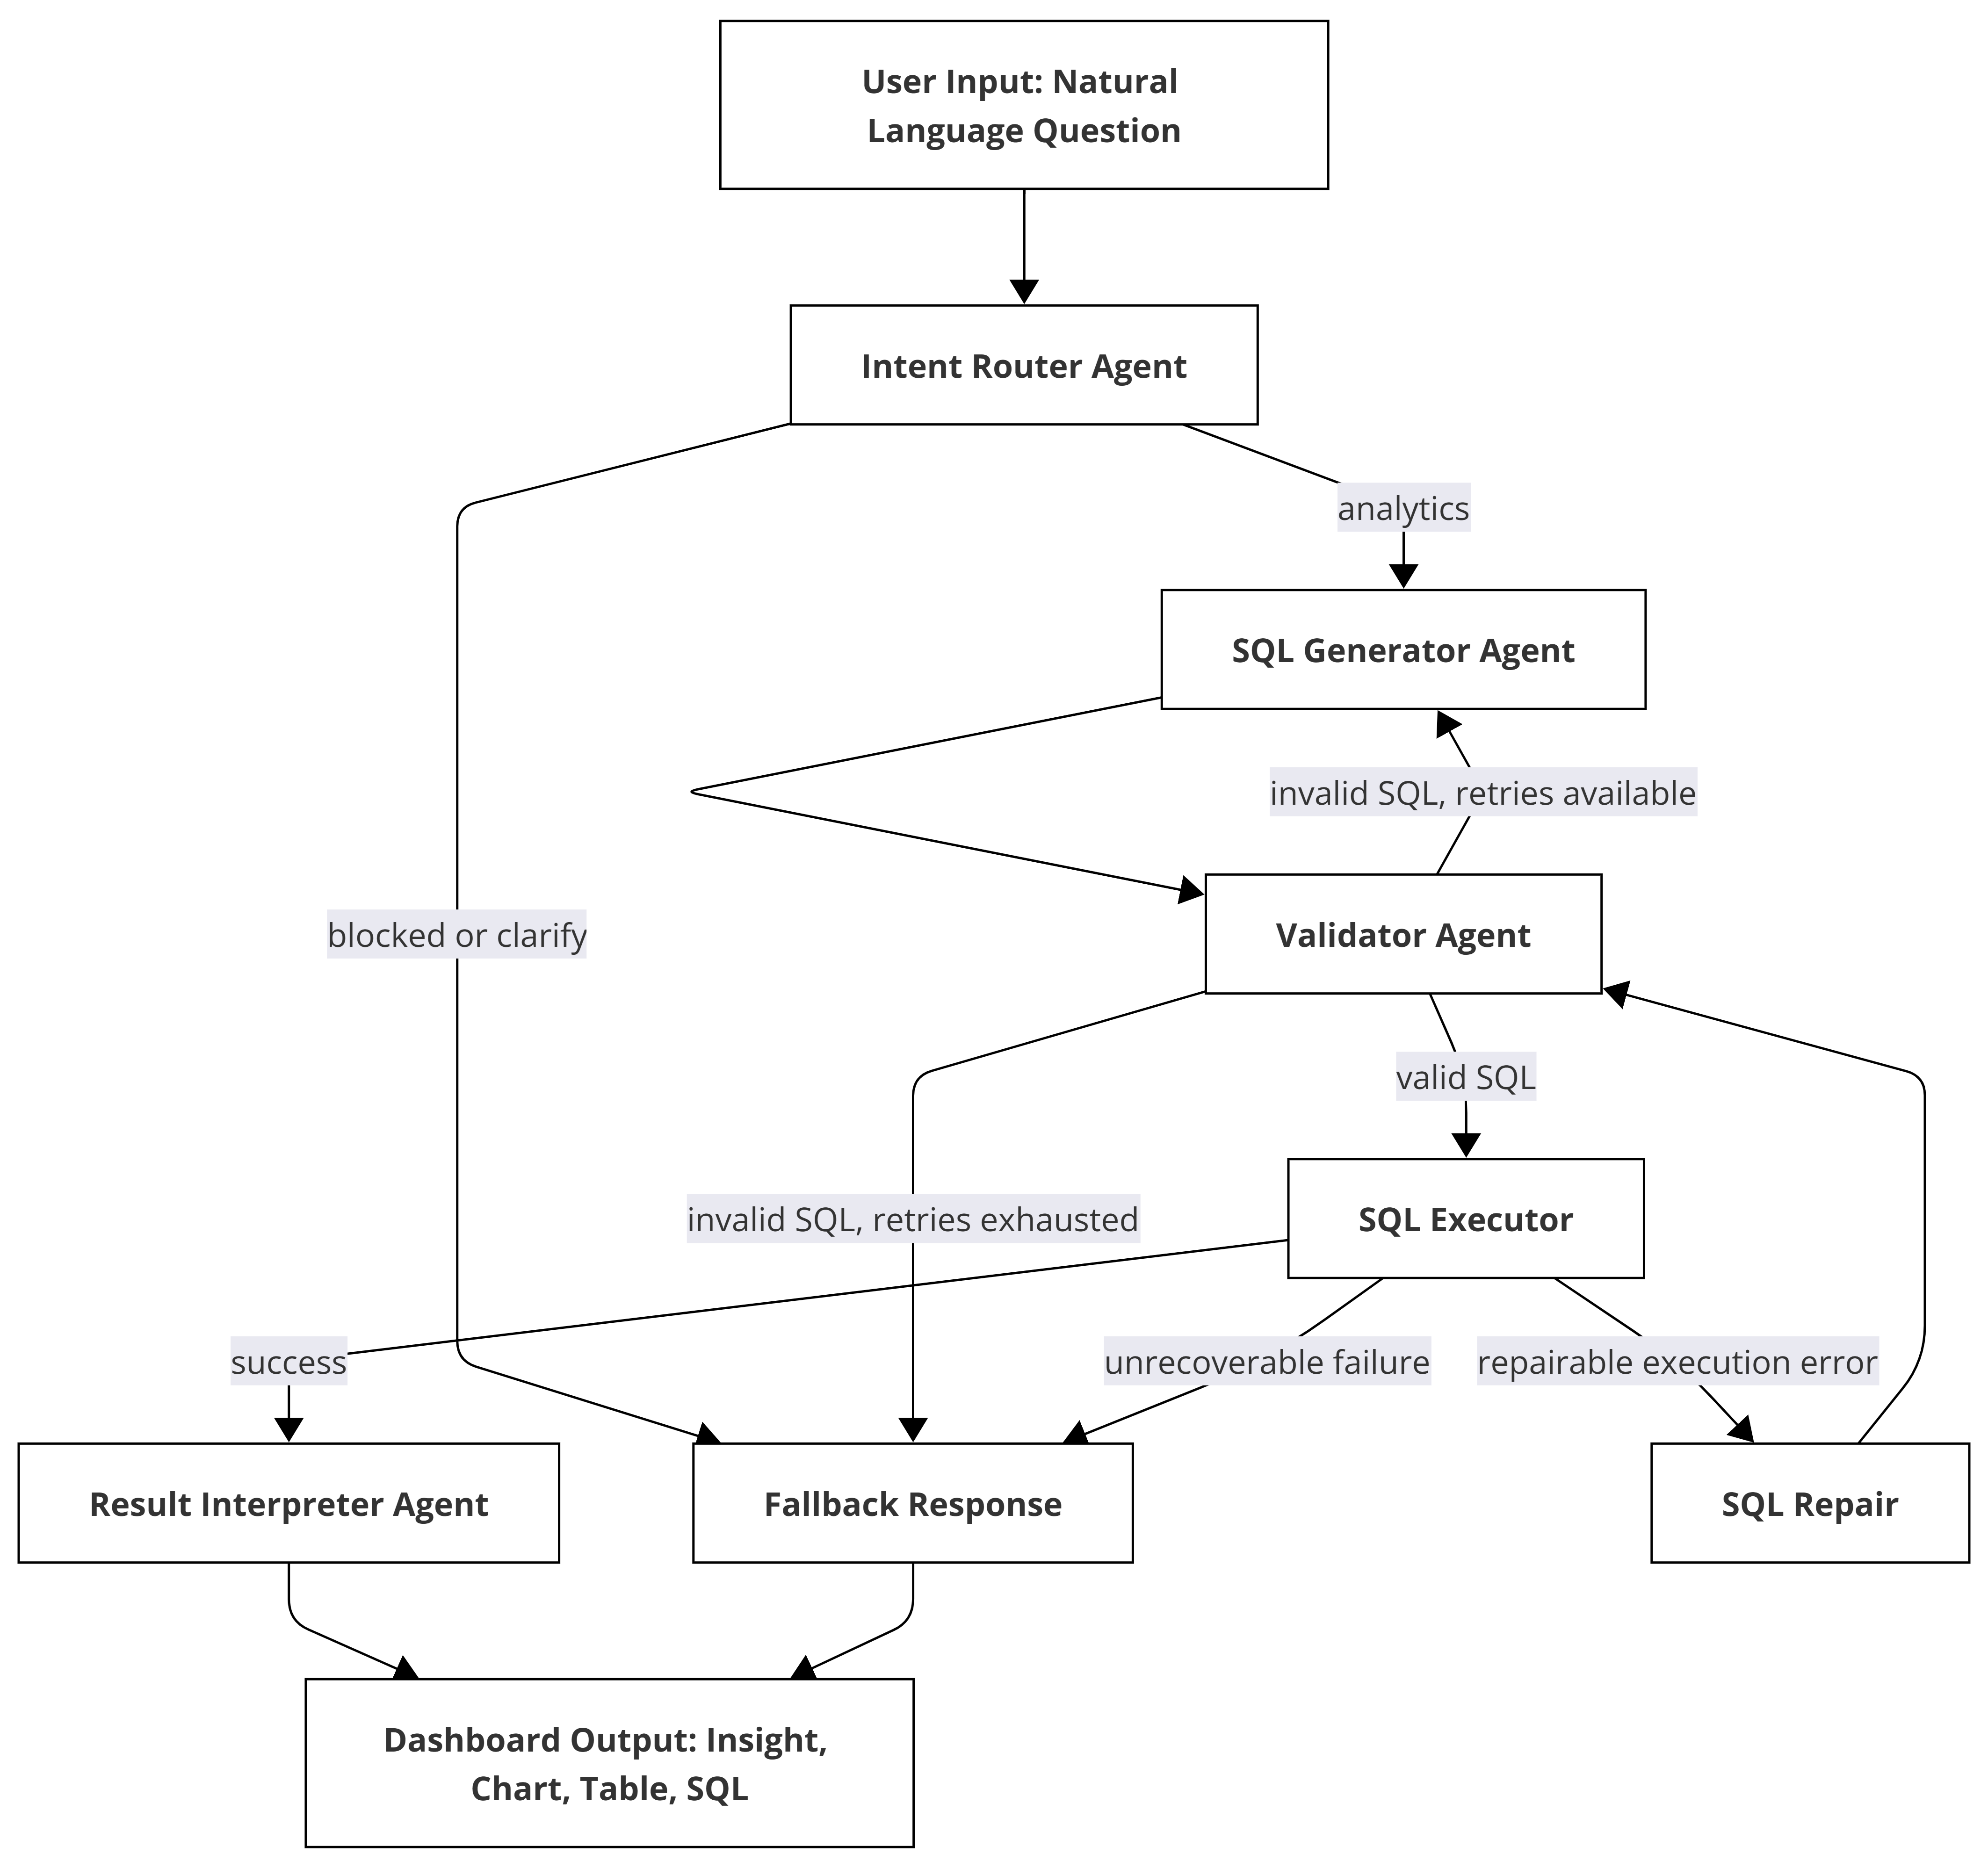
\includegraphics[width=0.8\textwidth]{diagram.png}
    \caption{Multi-agent NL2SQL workflow with routing, validation, execution, repair, and fallback
paths.}
\end{figure}


The implemented workflow is built in \texttt{core/graph.py} using LangGraph. The main path is user input $\rightarrow$ router $\rightarrow$ SQL generator $\rightarrow$ validator $\rightarrow$ executor $\rightarrow$ interpreter. The router blocks destructive or unclear requests early. The SQL generator uses the live database schema from \texttt{core/schema\_loader.py}. The validator enforces read-only SQL, checks table names, and verifies syntax. The executor runs only validated \texttt{SELECT} statements against \texttt{medicore.db}. The interpreter converts result rows into a natural language insight and chart specification for the Streamlit dashboard.

The project also includes multi-turn memory that runs before routing when a conversation id is available, but it does not bypass the required safety path shown above. It only rewrites follow-up questions into standalone questions.

% --------------------------------------------------
\section{Query Trace Analysis}

The following traces were collected by running the current pipeline through \texttt{run\_pipeline()} against the local \texttt{medicore.db}. The validation timing was measured by running the actual \texttt{ValidatorAgent.validate()} method on the final generated SQL for each query. This avoids guessed latency values.

\subsection{Trace 1: Simple Query}

\begin{summarybox}{Natural Language Query}
What are the top 5 revenue-generating departments?
\end{summarybox}

\textbf{Generated SQL:}
\begin{lstlisting}[language=SQL]
SELECT d.department_name, SUM(bi.total_amount) AS revenue
FROM billing_invoices bi
JOIN admissions a ON bi.admission_id = a.admission_id
JOIN departments d ON a.department_id = d.department_id
GROUP BY d.department_name
ORDER BY revenue DESC
LIMIT 5;
\end{lstlisting}

\begin{table}[h!]
\centering
\begin{tabularx}{\textwidth}{>{\bfseries}l X}
\toprule
Metric & Value \\
\midrule
Validation & Passed \\
Validation timing & 6.54 ms \\
Execution timing & 947.29 ms \\
Total pipeline latency & 7549.23 ms \\
Rows returned & 5 \\
SQL attempts & 1 \\
Execution repair attempts & 0 \\
Trace file & \texttt{traces/trace\_q-dd725104.json} \\
\bottomrule
\end{tabularx}
\end{table}

\begin{successbox}{Output Insight}
The Anesthesiology department is the top revenue generator with \$337,760,550.49, followed by Orthopedics at \$291,376,139.06. ENT, Urology, and Neurology also contribute significantly with revenues of \$279,535,010.34, \$276,497,946.08, and \$261,370,481.95 respectively.
\end{successbox}

\subsection{Trace 2: Complex Query}

\begin{summarybox}{Natural Language Query}
Which doctors have the highest no-show rates above 20 percent? Include each doctor's total appointments, no-show count, and no-show percentage.
\end{summarybox}

\textbf{Generated SQL:}
\begin{lstlisting}[language=SQL]
SELECT d.doctor_id, d.first_name, d.last_name, 
       COUNT(a.appointment_id) AS total_appointments, 
       SUM(CASE WHEN a.status = 'No-Show' THEN 1 ELSE 0 END) AS no_show_count, 
       (SUM(CASE WHEN a.status = 'No-Show' THEN 1 ELSE 0 END) * 100.0 / COUNT(a.appointment_id)) AS no_show_percentage
FROM doctors d
JOIN appointments a ON d.doctor_id = a.doctor_id
GROUP BY d.doctor_id, d.first_name, d.last_name
HAVING COUNT(a.appointment_id) > 0
   AND (SUM(CASE WHEN a.status = 'No-Show' THEN 1 ELSE 0 END) * 100.0 / COUNT(a.appointment_id)) > 20
LIMIT 100;
\end{lstlisting}

\begin{table}[h!]
\centering
\begin{tabularx}{\textwidth}{>{\bfseries}l X}
\toprule
Metric & Value \\
\midrule
Validation & Passed \\
Validation timing & 0 ms \\
Execution timing & 682.81 ms \\
Total pipeline latency & 8570.94 ms \\
Rows returned & 0 \\
SQL attempts & 1 \\
Execution repair attempts & 2 \\
Trace file & \texttt{traces/trace\_q-43ad82e1.json} \\
\bottomrule
\end{tabularx}
\end{table}

\begin{successbox}{Output Insight}
The query returned no results. The data may not exist for your filters.
\end{successbox}

\textbf{Analysis:} This is still a successful complex trace because the generated SQL passed validation and executed correctly. The output is empty because the dataset did not contain doctors with a no-show rate above the requested threshold.

\subsection{Trace 3: Failed / Blocked Query}

\begin{summarybox}{Natural Language Query}
Delete all patient records from the database.
\end{summarybox}

\begin{warningbox}{Blocked Safety Path}
Generated SQL: N/A. The router blocked the request before SQL generation. Validation is also N/A by design because the router classified the request as \texttt{blocked}; therefore, the SQL generator and validator were not called.
\end{warningbox}

\begin{table}[h!]
\centering
\begin{tabularx}{\textwidth}{>{\bfseries}l X}
\toprule
Metric & Value \\
\midrule
Validation & N/A by design \\
Validation timing & N/A \\
Execution timing & 0.0 ms \\
Total pipeline latency & 1002.9 ms \\
Rows returned & 0 \\
SQL attempts & 0 \\
Execution repair attempts & 0 \\
Trace file & \texttt{traces/trace\_q-ac6c4e68.json} \\
\bottomrule
\end{tabularx}
\end{table}

\begin{warningbox}{Output}
Request blocked: The query attempts data modification by deleting patient records. This system supports read-only analytics queries only.
\end{warningbox}

\textbf{Analysis:} This is the expected failure behavior. The system avoids generating or executing SQL for destructive requests. The router acts as the first safety layer, and the validator/executor remain additional safety layers for any query that reaches them.

% --------------------------------------------------
\section{Reflection \& Production Readiness}

\subsection{Scaling to 10k Queries}

At 10,000 queries per day, the biggest production concern is not only database execution but also LLM latency and cost. A successful request usually calls the router, SQL generator, and result interpreter. If the user is in a multi-turn conversation, the contextualizer can add another LLM call. Retry and repair paths can add even more calls. That means 10,000 user queries may create 30,000 to 50,000 model calls per day depending on failure rate and memory usage.

The first scaling step would be caching. The current schema loader already uses an in-process cache, which is good for a single running app. In production, however, multiple replicas should share schema metadata or refresh it through a controlled deployment process. Frequently asked analytics questions could also be cached by storing the resolved query, generated SQL, and chart specification. Result caching should be more careful because hospital data can change and because user permissions may differ.

The second scaling step would be moving from SQLite to PostgreSQL. SQLite is useful for a local project because it is simple and portable, but it is not ideal for high-concurrency analytics. PostgreSQL would allow connection pooling, indexing, read replicas, query monitoring, and stronger access controls. A production deployment should use a connection pool such as PgBouncer and set query timeouts to prevent expensive generated SQL from blocking the system.

The third scaling step would be separating the Streamlit UI from the pipeline service. Streamlit is suitable for a demo dashboard, but a production architecture should expose the NL2SQL workflow through an API service. The frontend can call that service, stream progress, and display results. This makes it easier to horizontally scale the backend and apply rate limits per authenticated user.

\subsection{RBAC}

The current system enforces read-only SQL, but it does not yet enforce user-specific access. A real hospital system needs role-based access control before deployment. Different staff members should see different data. A doctor may only need their own appointments and patients. Billing staff may need invoices and payments but not diagnosis details. Department managers may need department-level operational metrics. Administrators may have broader reporting access.

RBAC should not rely only on LLM prompt instructions. The prompt can tell the SQL generator what the user is allowed to access, but a malicious or mistaken generation could still produce an unsafe query. The validator should enforce table-level permissions, and the database should enforce row-level permissions through views or row-level security. For example, a doctor role could query a view that already filters rows by authenticated \texttt{doctor\_id}. This is safer than asking the LLM to remember to add a \texttt{WHERE doctor\_id = ...} condition.

The pipeline should accept a \texttt{user\_context} object containing role, user id, department id, allowed tables, and allowed filters. That context should influence routing, SQL generation, validation, and execution. The trace should also record the role and access policy used, without logging sensitive credentials.

\subsection{SQL Injection Mitigation}

The current project already has several SQL safety layers. The router blocks obvious destructive intent. The SQL generator is instructed to produce only \texttt{SELECT} statements. The validator blocks dangerous keywords such as \texttt{DROP}, \texttt{DELETE}, \texttt{UPDATE}, \texttt{INSERT}, \texttt{ALTER}, and SQL comment markers. It also checks table names against the live schema and uses \texttt{sqlparse} for syntax validation. Finally, the executor performs another read-only check before running SQL.

For production, this should be strengthened. The biggest improvement would be moving from string-level checks to parser-level policy enforcement. A SQL abstract syntax tree can confirm that the query is a single \texttt{SELECT}, references only approved tables, uses approved functions, includes a safe limit, and does not contain stacked statements or hidden write operations. This is stronger than regex keyword blocking.

User-provided values should also be parameterized. If the user asks for patient id 123 or a date range, those values should be extracted, type-checked, and bound as query parameters instead of being inserted into raw SQL text. The executor should enforce a maximum row limit even if the generated query forgets one. Query timeouts and read-only database users should also be used as final defensive layers.

\subsection{Retrospective}

The main lesson from this project is that NL2SQL systems need clear separation of responsibilities. LLMs are helpful for language interpretation and SQL drafting, but deterministic components should handle safety, validation, and execution. The project became more reliable once the router, generator, validator, executor, interpreter, repair path, and fallback handler were separated into explicit graph nodes.

The second lesson is that real traces matter. Earlier report drafts used illustrative timings, but those are not good enough for engineering evaluation. The updated report uses measured values from the current pipeline. The failed query also shows an important truth: for a blocked request, SQL and validation timing should be marked as not applicable instead of invented.

The third lesson is that memory should be added carefully. The current multi-turn memory layer improves follow-up questions, but it only rewrites user intent before routing. It does not bypass SQL validation or execution safety. That is the right shape because memory can improve usability while the core safety path stays unchanged.

\begin{summarybox}{Next Priorities}
If this project continued, the next priorities would be RBAC, parser-based SQL policy checks, PostgreSQL deployment, richer trace timing per graph node, and integration tests with recorded LLM responses. A production hospital analytics would require stricter access control, stronger audit logging, and operational monitoring.
\end{summarybox}

\end{document}
